\begin{figure}
  \centering
  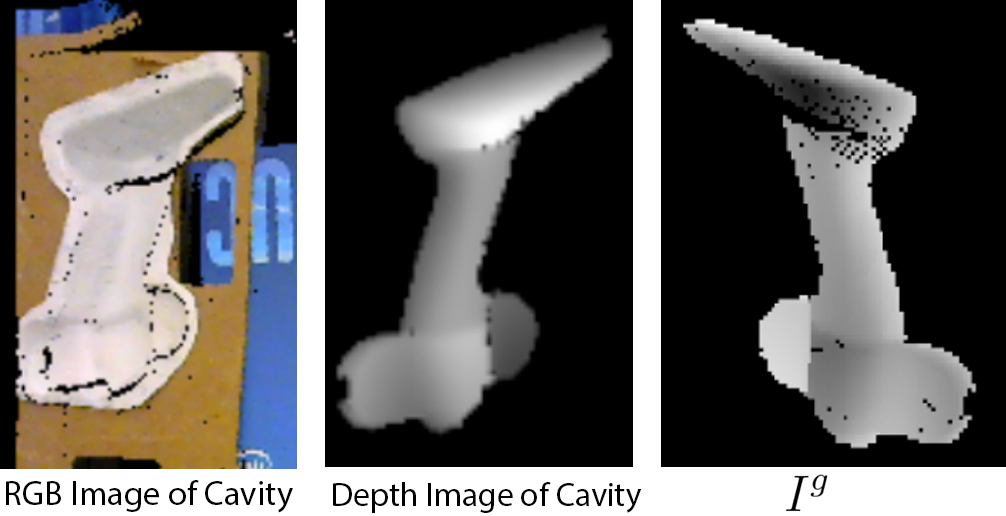
\includegraphics[width=0.48\textwidth]{figures/Rotated_Negative.png}
  \caption{\textbf{Generating Negative Goal Images: }After taking the original image (left), we segment out all parts that don't belong to the cavity (middle). Then, we project from depth to point cloud, rotate the pointcloud about its centroid, and deproject to depth image to get $I^g$ (right).}
  \label{fig:rotated-cavity}
\end{figure}
